\setlength{\columnsep}{3pt}
\begin{flushleft}
	
	The \textbf{fdisk} is started by typing (as root) fdisk device at the command prompt. 
	\bigskip
	\begin{tcolorbox}[breakable,notitle,boxrule=-0pt,colback=pink,colframe=pink]
		\color{black}
		\fontdimen2\font=1em
		Syntax: fdisk HDD\_device\_name
	\end{tcolorbox}

	\bigskip
	Eg:
	\begin{tcolorbox}[breakable,notitle,boxrule=-0pt,colback=black,colframe=black]
		\color{green}
		\fontdimen2\font=1em
		\# fdisk /dev/sda
		\fontdimen2\font=4pt
	\end{tcolorbox}
	
	To display all the device details using \textbf{fdisk} command with \textbf{"-l"} option:
	\bigskip
	\begin{tcolorbox}[breakable,notitle,boxrule=-0pt,colback=pink,colframe=pink]
		\color{black}
		\fontdimen2\font=1em
		Syntax: fdisk -l
		\fontdimen2\font=4pt
	\end{tcolorbox}
	
	
	More options for \textbf{fdisk} command:
	\begin{itemize}
				\item \textbf{p}: Print the partition table
				\item \textbf{n}: Create a new partition
				\item \textbf{d}: Delete a partition
				\item \textbf{q}: Quit without saving changes
				\item \textbf{w}: Write the new partition table and exit
	\end{itemize}
\newpage

\paragraph{Creating the primary partitions}

\begin{figure}[h!]
	\centering
	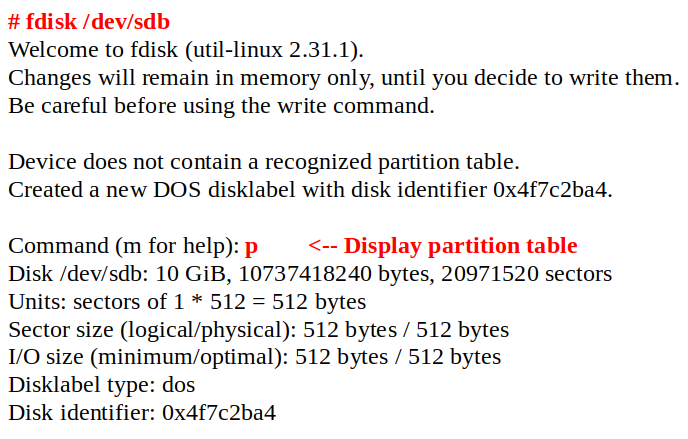
\includegraphics[scale=.4]{content/chapter8/images/fdisk1.png}
	\caption{fdisk 'p' option}
	\label{p_option}
\end{figure}		

\paragraph{Creating primary partition of size 1G}
\begin{figure}[h!]
	\centering
	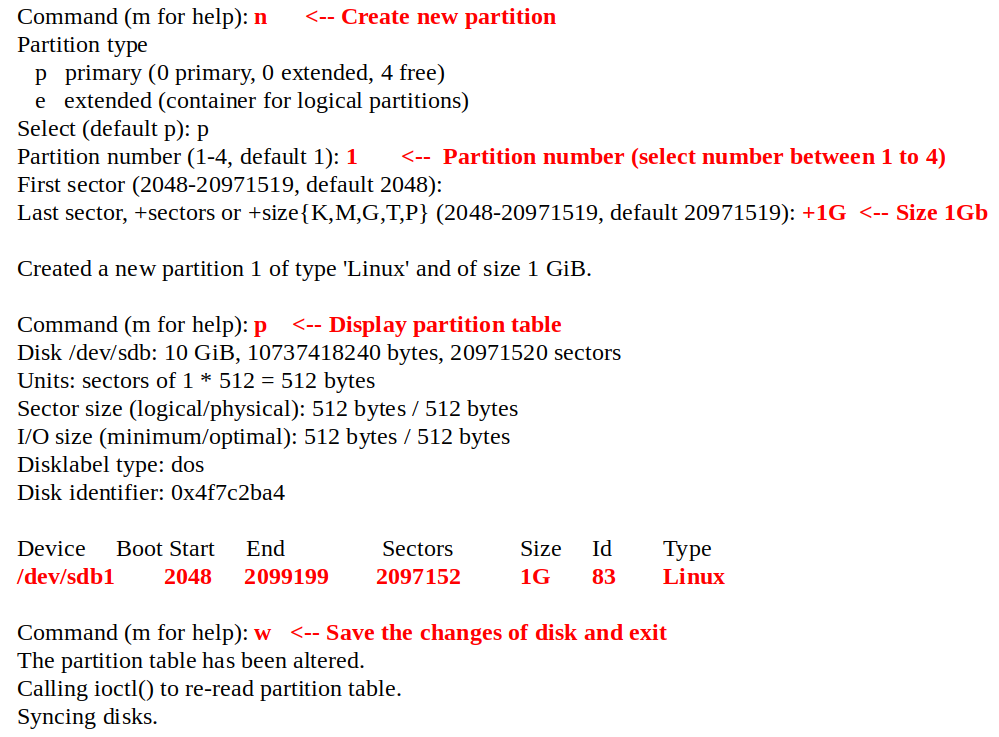
\includegraphics[scale=.4]{content/chapter8/images/fdisk2.png}
	\caption{fdisk 'n' \& 'w' option}
	\label{n_w_option}
\end{figure}		

\newpage
\paragraph{Creating the extended partitions of remaining size of disk}

\begin{figure}[h!]
	\centering
	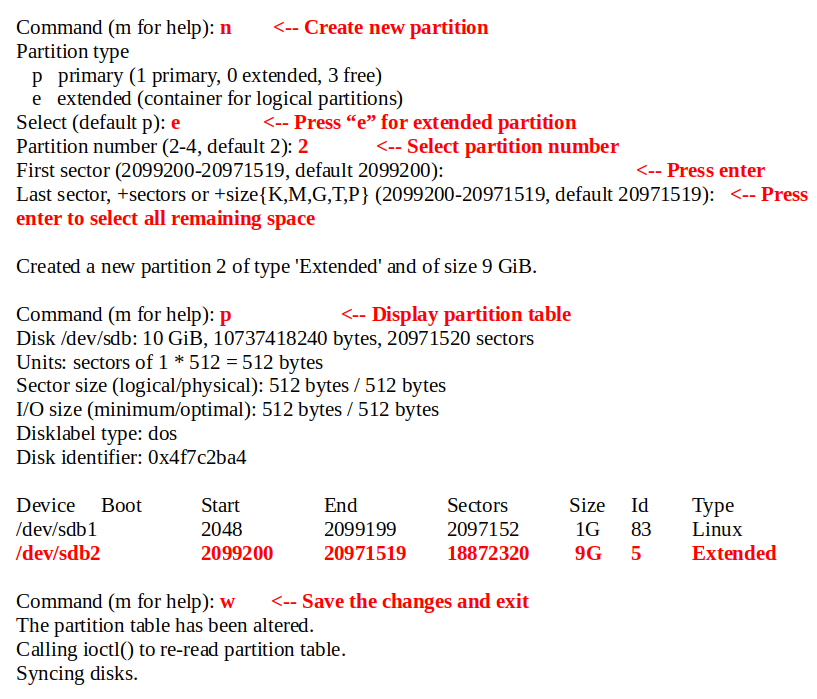
\includegraphics[scale=.5]{content/chapter8/images/fdisk3.png}
	\caption{fdisk 'e' option}
	\label{e_option}
\end{figure}		

\newpage
\paragraph{Creating the logical partitions of size 1G}

\begin{figure}[h!]
	\centering
	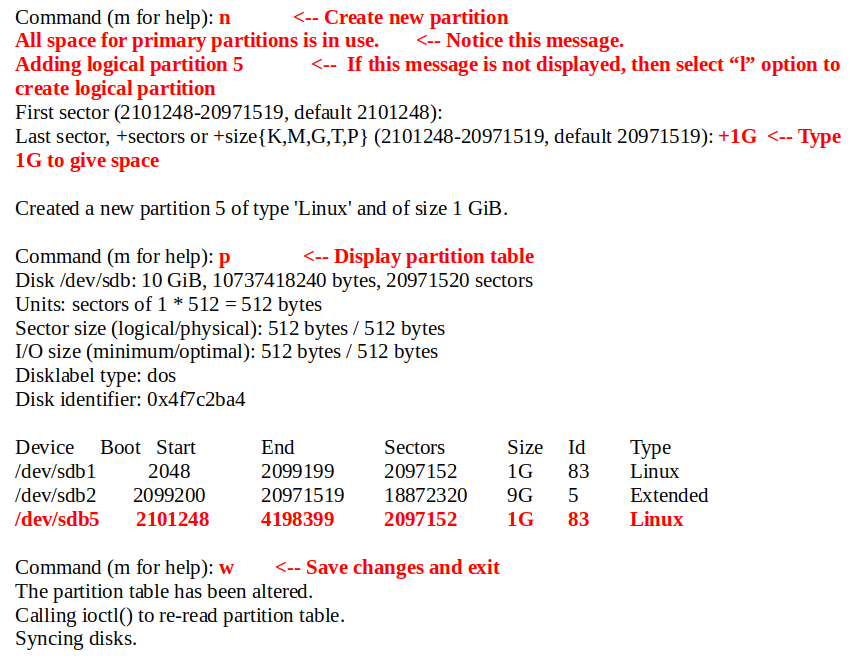
\includegraphics[scale=.5]{content/chapter8/images/fdisk5.png}
	\caption{fdisk 'l' option}
	\label{l_option}
\end{figure}		

\newpage

\paragraph{Deleting partition using fdisk command}
\begin{figure}[h!]
	\centering
	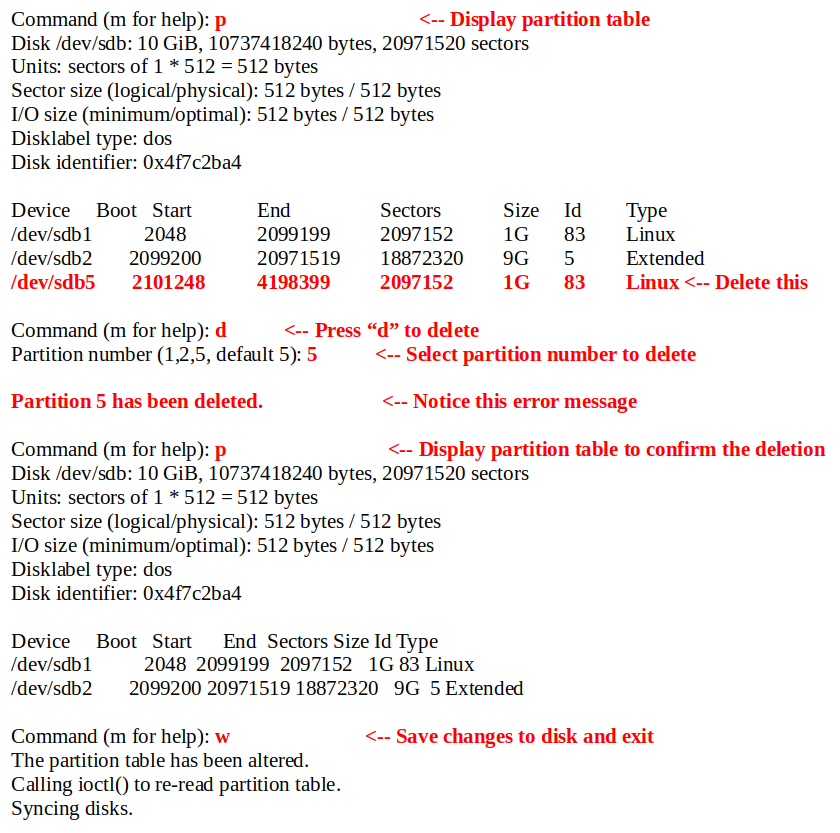
\includegraphics[scale=.5]{content/chapter8/images/fdisk6.png}
	\caption{fdisk 'd' option}
	\label{d_option}
\end{figure}		



\end{flushleft}

\newpage

